\chapter{Transmission Derivation}

This is an expanded version of the analysis performed for Fig.~\ref{fig:energydistrib}

\begin{equation}
T = T(\omega, x_o) = \frac{(\exp(-\frac{L}{\xi}))^2}{ 
(\omega-\omega _o)^2 + (\exp(-\frac{L}{\xi})\frac{1}{2}\exp(\frac{\mid L-2 x_o \mid}{\xi}))^2 }
\label{fig:appendixtransmission}
\end{equation}
Where we have appoximated cosh() as $\frac{1}{2}\exp()$. 

From the behavior of transmission in media with defects and centers of localizaiton, we see two cases when on a resonant frequency:  either the defect is in the first half of the sample.%, (\ref{fig:cononicaldefectpositions}, plot 1).

\begin{equation}
{\cal E}(x) = \left\{ 
\begin{array}{l l}
  A \exp\left(\frac{2 (x-x_o)}{\xi}\right) & \quad 0 < x < x_o \\
  B \exp\left(-\frac{2 (x-x_o)}{\xi}\right) & \quad x_o < x < L\\
\end{array} \right.
\label{fig:left}
\end{equation}

or it is in the second half of the sample.%, (\ref{fig:cononicaldefectpositions}, plot 2).
\begin{equation}
{\cal E}(x) = \left\{ 
\begin{array}{l l}
 A \exp\left(-\frac{2 x}{\xi}\right) & \quad 0 < x < L-2 x_o \\
 B \exp\left(\frac{2 (x-x_o)}{\xi}\right) & \quad L-2 x_o < x < x_o \\
 C \exp\left(-\frac{2 (x-x_o)}{\xi}\right) & \quad x_o < x < L \\
\end{array} \right.
\label{fig:right}
\end{equation}

With either case, we see three distinct regions when the frequency is not on resonance but prior to the pure exponential decay regimes. %(\ref{fig:cononicaldefectpositions}, plot 3):
\begin{equation}
{\cal E}(x) = \left\{ 
\begin{array}{l l}
y_1 = A \exp\left(-\frac{2 x}{\xi}\right)   & \quad 0 < x < x_1  \\
y_2 = B \exp\left(\frac{2 (x-x_o)}{\xi}\right) & \quad x_1 < x < x_o  \\
y_3 = C \exp\left(-\frac{2 (x-x_o)}{\xi}\right) & \quad  x_o < x < L \\
\end{array} \right.
\label{fig:startingequations}
\end{equation}
Where $x_1$ is the turning point.

\begin{comment}
%% pictures were removed, causes a problem during compile (?)
\begin{figure}
\vskip -0.5cm
\centerline{
\scalebox{0.5}{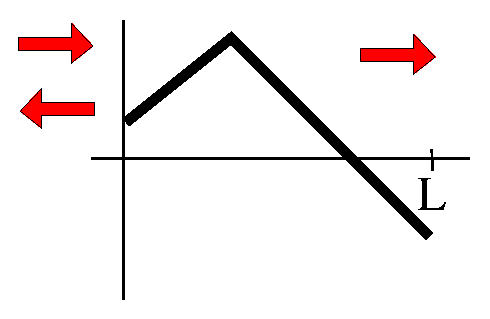
\includegraphics{pictures/transmission_derivation_14_LR}}
\scalebox{0.5}{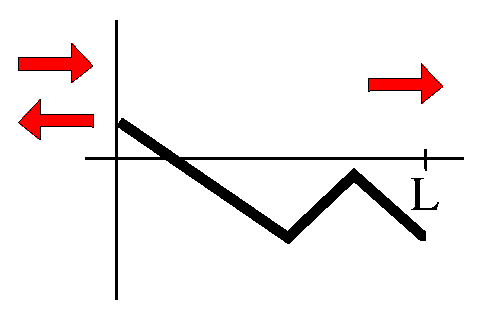
\includegraphics{pictures/transmission_derivation_34_LR}}
\scalebox{0.5}{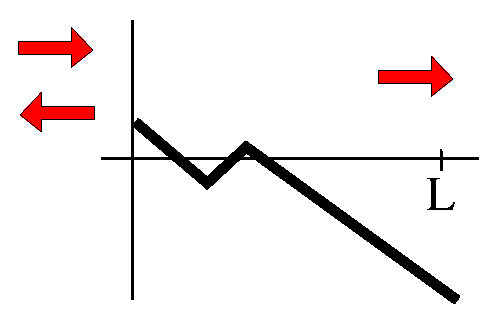
\includegraphics{pictures/transmission_derivation_off_res_LR}}
}
\vskip -0.5cm
\caption{Log of energy versus position sketches for a center of localization in the first half (left), Eq.~\ref{fig:left}; and second half (center), Eq.~\ref{fig:right}. The turning point in the center plot is $L-2 x_o$. The right sketch is off-resonance but prior to pure exponential decay, which applies to any center of localization position, as described by Eq.~\ref{fig:startingequations}. The turning point in the right plot from the initial exponential decay to growth varies depending how far off resonance one is. We call this $x_1$}
\label{fig:cononicaldefectpositions}
\end{figure}
\end{comment}

From the off-resonance Eq.~\ref{fig:startingequations}, we apply boundry conditions to determine the coefficients in passive systems. We take gain into account and make corrections later.

At $x=0$ then $y_1=4$, giving $A=4$. Thus
\begin{equation}
\boxed{y_1 = 4 \exp\left(-\frac{2 x}{\xi}\right)}   \quad \quad \quad 0 < x < L-2 x_o 
\end{equation}

At $x=L$, $y_3=T$. Solve for C,
\begin{equation}
C=T \exp\left(\frac{2(L-x_o)}{\xi}\right)
\end{equation}
plug back in,
\begin{equation}
y_3 = T \exp\left(\frac{2(L-x_o)}{\xi}) \exp(-\frac{2 (x-x_o)}{\xi}\right)  \quad \quad \quad  x_o < x < L
\end{equation}
simplify to get
\begin{equation}
\boxed{y_3 = T \exp\left(-\frac{2(x-L)}{\xi}\right)}  \quad \quad \quad  x_o < x < L
\end{equation}
at $x_o$, $y_2 = y_3$
\begin{equation}
B \exp\left(\frac{2 (x_o-x_o)}{\xi}\right) = B = T \exp\left(-\frac{2(x_o-L)}{\xi}\right)
\end{equation}
plug in to $y_2$
\begin{equation}
y_2 = T \exp\left(-\frac{2(x_o-L)}{\xi}\right) \exp\left(\frac{2 (x-x_o)}{\xi}\right) \quad \quad \quad L-2 x_o < x < x_o 
\end{equation}
simplify to get
\begin{equation}
\boxed{y_2 = T \exp\left(\frac{2(x+L-2 x_o)}{\xi}\right)} \quad \quad \quad L-2 x_o < x < x_o 
\end{equation}

The turning point $x_1$ varies as a function of frequency. Boundry conditions on $x_1$ are that it should remain less than $x_o$ and that it be non-negative. To solve for $x_1$, see where $y_1=y_2$
\begin{equation}
4 \exp\left(-\frac{2 x_1}{\xi}\right) = T \exp\left(\frac{2(x_1+L-2 x_o)}{\xi}\right)
\end{equation}

\begin{equation}
\boxed{x_1(\omega) = -\frac{\xi}{4} \log(\frac{1}{4} T) - \frac{1}{2}L + x_o}
\end{equation}

Knowing $y_1,y_2$, and $y_3$ we can integrate to find the energy ${\cal E}$:
\begin{equation}
\begin{gathered}
{\cal E}(x,\omega) = \int _0 ^{x_1} 4 \exp\left(-\frac{2 x}{\xi}\right) dx +
    \int _{x_1} ^{x_o} T \exp\left(\frac{2(x+L-2 x_o)}{\xi}\right) dx + \\
    \int _{x_o} ^{L} T \exp\left(-\frac{2(x-L)}{\xi}\right)
\label{fig:Eintegral}
\end{gathered}
\end{equation}

Solve, reduce to get the energy as a function of x, frequency, and transmission:
\begin{equation}
\begin{gathered}
{\cal E}(x,\omega) = \frac{\xi}{2} \left( T \left( \exp\left(\frac{2(L-x_o)}{\xi}\right) - \exp\left(\frac{2(L-2 x_o+x_1)}{\xi}\right)+\right. \right.\\
\left.\left.\exp\left(\frac{2(L-x_o))}{\xi}\right) -1 \right) + 4 \left(1-\exp\left(-\frac{2 x_1}{\xi}\right)\right) \right)
\label{fig:appendixenergy}
\end{gathered}
\end{equation}

